\section{Pixelation Patterns of ViT-VQGAN} \label{secs:appendix_pixelation}

\begin{figure}[!ht]
\centering
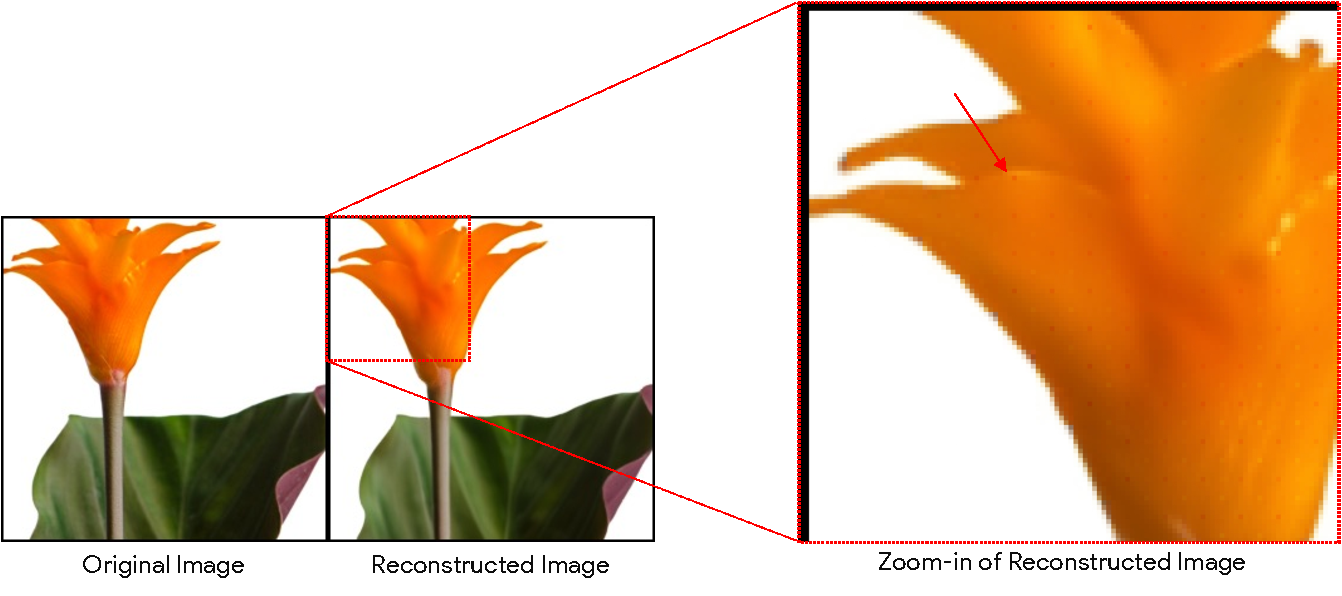
\includegraphics[width=0.8\textwidth]{figures/pixelation.pdf}
\caption{Example of pixelation patterns (saturated pixel values at  some locations) in the outputs of ViT-VQGAN~\cite{yu2021vector} architecture when zooming in. It can be fixed by removing the final sigmoid activation layer and the logit-laplace loss, exposing the raw values as RGB pixel values (in range [0, 1]).}
\label{figs:pixelation}
\end{figure}

We notice visual pixelation patterns in some of the output images of ViT-VQGAN when zooming in (see Appendix~\ref{secs:appendix_pixelation}), and further find ill-conditioned weight matrices of the output projection layer before the sigmoid activation function. As a fix, we remove the final sigmoid activation layer and the logit-laplace loss, exposing the raw values as RGB pixel values (in range [0, 1]). Conveniently, this fix can be hot-swappable into an already trained image tokenizer by finetuning the decoder.